Kako bismo bolje približili pojam apstraktne interpretacije, koristićemo se
optimizacijskom tehnikom koju prevodioci koriste zvanu \emph{propagacija konstanti}.
Sam proces propagacije konstanti se svodi na menjanje promenljivih u izrazima
konstantnim vrednostima, u slučaju kada njihove vrednosti ne zavise niti od
ulaznih parametara funkcije, niti od dela koda koji se izvršavao u toj funkciji.
\lstinputlisting[language=C++, caption=Kod sa grananjem, label=ex1]{snippets/ex1.cpp}

\subsection{Grafovi kontrole toka}
\label{subsec:cfgs}

\begin{figure}[H]
\begin{center}
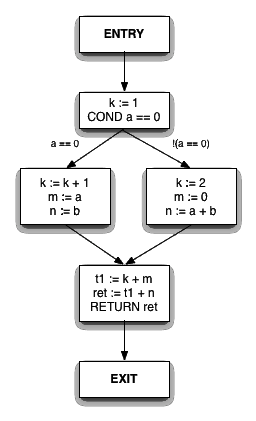
\includegraphics[scale=0.5]{Treehydra-cfg.png}
\end{center}
\caption{Primer grafa kontole toka}
\label{fig:graf}
\end{figure}

Svaki deo koda \ref{ex1} se može predstaviti \emph{grafom kontrole toka (eng. control flow graph, CFG)},
i upravo takva reprezentacija će se koristiti za opis apstraktne interpretacije.
Slika \ref{fig:graf} prikazuje funkciju predstavljenu na ovaj način, koju ćemo koristiti za
opis ovog metoda statičke analize.

Neke napomene:
\begin{itemize}
\item Veze između čvorova grafa su predstavljene kao grane, pojavljuju se u sluča\-ju
kada imamo naredbe kontrole toka (petlje, uslovni/bezuslovni skokovi itd.).
\item Naredbe imaju najviše jednu dodelu i tačno jednu operaciju. U slučaju naredbe
sa više operacija, vršimo razdvajanje na naredbe sa po jednom operacijom, čije
ćemo rezultate čuvati u pomoćnim promenljivama.
\end{itemize}

Terminologije:
\begin{itemize}
\item Svaki čvor se zove \textbf{osnovni blok} \emph{(eng. basic block, \textbf{BB})}.
Osnovni blok se definiše tako što ima samo jednu tačku ulaza, i jednu tačku izlaza,
što će reći da nema grananja unutar osnovnih blokova.
\item Naredbe ćemo zvati \emph{instrukcije}, iako one uopšteno mogu imati
različite nazive u zavisnosti od toga koliko operanada primaju.
\item \textbf{Tačka u programu} je zamišljena tačka pre ili posle svake instrukcije.
Funkcija ima dobro definisano stanje u svakoj tački, tako da će se naša analiza
programa uvek referisati na ove tačke.
\end{itemize}


\subsection{Konkretna interpretacija}
\label{subsec:concreteimpr}
Pre nego što prođemo kroz primer koji opisuje proces apstraktne interpretacije,
napravićemo jedan prolaz kroz funkciju koju ispitujemo koristeći konkretne vrednosti
kao ulaz. Pritom ćemo pratiti promenljive unutar funkcije, obraćajući pažnju na
one koje su zadržale istu vrednost tokom izvršavanja. Uzmimo sledeće vrednosti za ulaz
\texttt{a = 0, b = 7}:
\verbatiminput{snippets/ex2_1.txt} 
Dakle, \texttt{k = 2} pre nego što se koristi u naredbi \texttt{t1 := k + m}.
Možemo pokrenuti funkciju za ostale ulaze i dobili bismo isti rezultat.
Međutim, ovakav način testiranja nam ne može potvrditi da je \texttt{k = 2} za
sve moguće ulaze. (Doduše može, ali samo ako bismo proverili sve moguće vrednosti
koje promenljiva može da uzme.)


\subsection{Približavanje apstraktnoj interpretaciji}
\label{subsec:approachingabsint}
Obratimo pažnju da za \texttt{k}, u okviru funkcije imamo dve bitne provere:
\texttt{a == 0} i \texttt{a != 0}, dok nam vrednost za \texttt{b} u ovom slučaju
nije bitna. Sada ćemo ispitati vrednost promenljivih u okviru funkcije za dva ulaza:
jedan sa ulazom \texttt{a = 0, b = ?}, a drugi sa ulazom \texttt{a = NN, b = ?},
gde \texttt{NN} označava ne-nula vrednost, dok \texttt{?} označava bilo koju vrednost.
Počnimo sa \texttt{a = 0, b = ?}:
\verbatiminput{snippets/ex2_2.txt}
Primetimo da nam se sada pojavljuju \texttt{NN} i \texttt{?}, apstraktne vrednosti
koje predstavljaju skupove konkretnih vrednosti.
Ostaje još da utvrdimo kako se ponašaju operatori nad apstraktnim vrednostima.
Na primer, u poslednjem koraku, \texttt{ret := t1 + n} postaje \texttt{ret := 2 + ?}.
Kako bismo saznali šta ovo znači, posmatramo skupove konkretnih vrednosti: Ako \texttt{?}
može biti bilo koja vrednost, onda i \texttt{2 + ?} takođe može uzeti bilo koju vrednost,
tako da \texttt{2 + ? $\longrightarrow$ ?}. Preostali slučaj testira \texttt{a = NN, b = ?}:
\verbatiminput{snippets/ex2_3.txt}
Posle ovog koraka se vidi da su pokriveni svi mogući ulazi, kao i svaki deo koda
funkcije, stoga možemo zaključiti da je \texttt{k = 2} uvek tačno pre nego što
dođemo do naredbe \texttt{t1 := k + m}.

Procedura koju smo upravo ispratili daje određen uvid kako bismo krenuli u proces
apstraktne interpretacije, ali nismo generalizovali samu proceduru. Tačno smo
znali koje apstraktne vrednosti da koristimo za test slučajeve, i to smo mogli
samo zato što smo imali kao primer jednostavnu funkciju. Ova metoda neće biti
primenjiva na komplikovane funkcije, i nije automatizovana.

Drugi problem je što smo posmatrali svaku granu funkcije posebno. Funckija sa \texttt{k} iskaza može imati i do
\texttt{$2^k$} grana, dok funkcija sa petljama ih može imati i beskonačno, i ovo nam onemogućava da imamo kompletnu
pokrivenost.

\subsection{Apstraktna interpretacija kroz primer}
\label{subsec:absintex}
Pre nego što krenemo u sam proces apstraktne interpretacije, treba da odaberemo
skupove apstraktnih vrednosti. Ponekad ne znamo kako da odaberemo skupove takvih
vrednosti, tako da ćemo sada proći kroz funkciju bez odabira ikakvih vrednosti:
Dakle, pokušajmo sa sledećim ulazom: \texttt{a = ?, b = ?}:
\verbatiminput{snippets/ex2_4.txt}
Pošto nemamo informaciju o tome šta je \texttt{a}, krenućemo put obe grane.
Prvo za potvrdnu granu:
\verbatiminput{snippets/ex2_5.txt}
Potom za negativni slučaj:
\verbatiminput{snippets/ex2_6.txt}
U ovoj tački, dva izvršna toka se spajaju. Mogli bismo da nastavimo da ih testiramo
ponaosob, ali znamo da će to dovesti do eksplozije u uopštenom slučaju, tako da ćemo
izvršiti spajanje stanja. Potrebno nam je jedno stanje koje pokriva obe grane:
\verbatiminput{snippets/ex2_7.txt}
Ovo stanje možemo dobiti tako što ćemo spajati promenljivu po promenljivu. Na primer,
\texttt{k} je 2 u jednom i u drugom stanju, tako da je \texttt{k = 2} u rezultujućem
stanju. Za \texttt{m}, ono može biti bilo šta u prvom stanju, tako da iako je ono 0
u drugom stanju, može uzeti bilo koju vrednost u rezultujućem stanju. Kao rezultat dobijamo:
\verbatiminput{snippets/ex2_8.txt}
Možemo nastaviti izvršavanje u jednom toku:
\verbatiminput{snippets/ex2_9.txt}
Gde dobijamo odgovor koji smo želeli, \texttt{k = 2}. Osnovne ideje su bile:
\begin{itemize}
\item Proći kroz funkciju koristeći apstraktne vrednosti kao ulaz
\item Apstraktna vrednost predstavlja skup konkretnih vrednosti
\item Kod kontrole toka gde imamo grananje, krenimo put obe grane
\item Gde imamo spajanje, spajamo izlaz iz obe grane
\end{itemize}
\cite{MozWiki}

\subsection{Primer upotrebe operatora proširenja}
\label{subsec:widening}

Razmotrimo sada primer \ref{ex3}. Jasno je da naša analiza ne može proći kroz petlju svih 10000 puta, u opštem slučaju mi ni ne možemo znati postoji li izlaz iz date petlje. Zato je potrebno upotrebiti operator proširenja pomenut u potpoglavlju \ref{subsec:widop}, u ovom slučaju takav da se desni kraj intervala proširi do beskonačnosti što nam daje fiksnu tačku operacije koja se izvršava unutar petlje. 

\lstinputlisting[language=C, caption=Kod sa petljom, label=ex3, showlines=true]{snippets/ex3.cpp}

Na kraju, dobijena stanja ograničavamo uslovom petlje koji zahteva da se $x$ nalazi unutar $(-\infty, 10000)$ na početku petlje a unutar $[10000, +\infty)$ na njenom izlazu. U tabeli \ref{tab:tabela1} prikazane su vrednosti dobijene u toku apstraktne interpretacije. \footnote{Primer je preuzet iz \cite{boulanger}}


\begin{table}[H]
\begin{center}
\caption{Apstraktne vrednosti promenljive x po linijama koda i koracima apstraktne interpretacije.}
\begin{tabular}{|l|l|l|l|l|l|} \hline
stanje& početak& prvi prolaz & drugi prolaz & proširenje & uslov\\ \hline
$x_1$ & $(-\infty, +\infty)$ & $(-\infty, +\infty)$ & $(-\infty, +\infty)$ & $(-\infty, +\infty)$ & $(-\infty, +\infty)$ \\ 
$x_2$ & $[\:]$ & $[1,1]$ & $[1,1]$ & $[1,1]$ & $[1,1]$ \\
$x_3$ & $[\:]$ & $[1,1]$ & $[1,3]$ & $[1,+\infty)$ & $[1,9999]$ \\
$x_4$ & $[\:]$ & $[3,3]$ & $[3,5]$ & $[3,+\infty)$ & $[3,10001]$ \\
$x_5$ & $[\:]$ & $[\:]$ & $[\:]$ & $[\:]$ & $[10000,10001]$ \\ \hline
\end{tabular}
\label{tab:tabela1}
\end{center}
\end{table}

